\documentclass[twoside,10pt]{article}

%================================ PREAMBLE ==================================

%--------- Packages -----------
\usepackage{fullpage}
\usepackage{amssymb}
\usepackage{amsmath}
\usepackage{amsthm}
\usepackage{latexsym}
\usepackage{graphicx}
\usepackage{color}
\usepackage{url}
\usepackage{listings}
\usepackage{pdfpages}
\usepackage{epstopdf}

%\usepackage{algorithm,algorithmic}

%----------Spacing-------------
%\setlength{\oddsidemargin}{0.25 in}
%\setlength{\evensidemargin}{-0.25 in}
\setlength{\topmargin}{-0.6 in}
%\setlength{\textwidth}{6.5 in}
%\setlength{\textheight}{9.4 in}
\setlength{\headsep}{0.75 in}
\setlength{\parindent}{0 in}
\setlength{\parskip}{0.1 in}

%----------Header--------------
\newcommand{\psetsubmission}[2]{
   \pagestyle{myheadings}
   \thispagestyle{plain}
   \newpage
   \setcounter{page}{1}
   \noindent
   \begin{center}
   \framebox{
      \vbox{\vspace{2mm}
    \hbox to 6.28in { {\bf ESE 542: Statistics for Data Science} \hfill {\bf Spring 2019} }
       \vspace{6mm}
       \hbox to 6.28in { \hfill {HW #1} \hfill }
       \vspace{6mm}
       \hbox to 6.28in { Name: \emph{#2} \hfill }
      \vspace{2mm}}
   }
   \end{center}
   \markboth{ESE 542: Statistics for Data Science, Spring 2019, HW}{#1}
   \vspace*{4mm}
}

%--------Environments----------
\theoremstyle{definition}
\newtheorem{thm}{Theorem}[section]
\newtheorem{lem}[thm]{Lemma}
\newtheorem{prop}[thm]{Proposition}
\newtheorem{cor}[thm]{Corollary}
\newenvironment{pf}{{\noindent\sc Proof. }}{\qed}
\newenvironment{map}{\[\begin{array}{cccc}} {\end{array}\]}

\theoremstyle{definition}
\newtheorem*{defn}{Definition}
\newtheorem{exmp}{Example}
\newtheorem*{prob}{Problem}
\newtheorem*{exer}{Exercise}

\theoremstyle{remark}
\newtheorem*{rem}{Remark}
\newtheorem*{note}{Note}

%---------Definitions----------
\newcommand{\Fig}[1]{Figure~\ref{#1}}
\newcommand{\Sec}[1]{Section~\ref{#1}}
\newcommand{\Tab}[1]{Table~\ref{#1}}
\newcommand{\Tabs}[2]{Tables~\ref{#1}--\ref{#2}}
\newcommand{\Eqn}[1]{Eq.~(\ref{#1})}
\newcommand{\Eqs}[2]{Eqs.~(\ref{#1}-\ref{#2})}
\newcommand{\Lem}[1]{Lemma~\ref{#1}}
\newcommand{\Thm}[1]{Theorem~\ref{#1}}
\newcommand{\Cor}[1]{Corollary~\ref{#1}}
\newcommand{\App}[1]{Appendix~\ref{#1}}
\newcommand{\Def}[1]{Definition~\ref{#1}}
%
\renewcommand{\>}{{\rightarrow}}
\renewcommand{\hat}{\widehat}
\renewcommand{\tilde}{\widetilde}
\newcommand{\half}{\frac{1}{2}}
%
\newcommand{\R}{{\mathbb R}}
\newcommand{\Z}{{\mathbb Z}}
\newcommand{\N}{{\mathbb N}}
\renewcommand{\P}{{\mathbf P}}
\newcommand{\E}{{\mathbf E}}
\newcommand{\Var}{{\mathbf{Var}}}
\newcommand{\I}{{\mathbf I}}
\newcommand{\1}{{\mathbf 1}}
\newcommand{\0}{{\mathbf 0}}
%
\newcommand{\sign}{\textup{\textrm{sign}}}
\newcommand{\er}{\textup{\textrm{er}}}
\newcommand{\abs}{\textup{\textrm{abs}}}
\newcommand{\sq}{\textup{\textrm{sq}}}
\newcommand{\zo}{\textup{\textrm{0-1}}}
%
\renewcommand{\H}{{\mathcal H}}
\newcommand{\F}{{\mathcal F}}
\newcommand{\X}{{\mathcal X}}
\newcommand{\Y}{{\mathcal Y}}
\newcommand{\bX}{{\mathbf X}}
%
\newcommand{\p}{{\mathbf p}}
\newcommand{\q}{{\mathbf q}}
\renewcommand{\r}{{\mathbf r}}
\newcommand{\x}{{\mathbf x}}
\newcommand{\y}{{\mathbf y}}
\renewcommand{\u}{{\mathbf u}}
\newcommand{\w}{{\mathbf w}}
%
\newcommand{\bloss}{{\boldsymbol \ell}}
\newcommand{\balpha}{{\boldsymbol \alpha}}
\newcommand{\bxi}{{\boldsymbol \xi}}
\newcommand{\bpsi}{{\boldsymbol \psi}}
\newcommand{\btau}{{\boldsymbol \tau}}


%=============================== END PREAMBLE ===============================

%============================ BEGIN DOCUMENT ================================

\begin{document}

%Use the following format: \psetsubmission{problem set number}{name}

\psetsubmission{5}{Tyler Olivieri}

%-------------------------------------------------- List Collaborators --------------------------------------------------

%\newpage
%--------------------------------------------- Begin Problem Solutions  --------------------------------------------


\begin{enumerate}

\item

  \begin{enumerate}

  \item

    The model summary shows $\beta _0 = 30.9787$ and $\beta_1 = -.12$, $\beta_1$ is just the slope of the line in the linear model. It explains the rate of change of the price with age. or the average effect on price of one unit increase in age. The hypothesis test corresponding to $\beta_1$ has the null hypothesis that $\beta_1 = 0$ (no relationship between age and price). With a p-value of 0, we reject this hypothesis with any significance, meaning there is certainly a relationship ($\beta_1 \neq 0$).
    
  \item

     The $R^2$ value is $.363$, meaning that the model did not approximate the real data very well. There is a lot of variance in the data not explained by the model.

  \item

    There are two parameters $\beta_0$ and $\beta_1$. The residual degrees of freedom is n-2 (the 2 comes from 2 parameters). It is the dimension of the space of the residuals. The residuals are constrained by two equations $\hat{e}_1 + ... + \hat{e}_n = 0$ and $x_1 \hat{e}_1 + ... + x_n  \hat{e}_n = 0$, then we have n-2 degrees of freedom. The residuals form a space of dimension n-2.
    
  \item

    I expect the residuals to be without a strong pattern for a linear (true) model. A pattern in the residuals would indicate some non-linearity in the data. I do not see much of a pattern, perhaps it is not centered around 0, but the residuals have high variance and a K-S test shows that that the residuals are not distributed normally.

  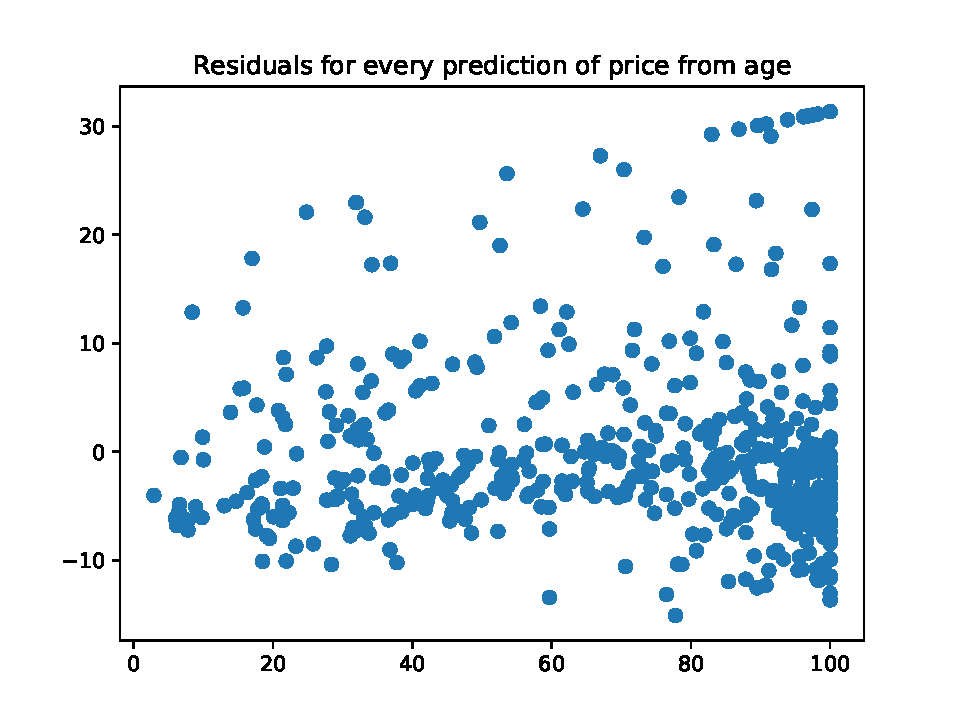
\includegraphics{hw5_1_d.pdf}
    
  \item

    If the model is true, I expect the probability plot to be directly on the linear line. However, we see that is not quite the case here.

  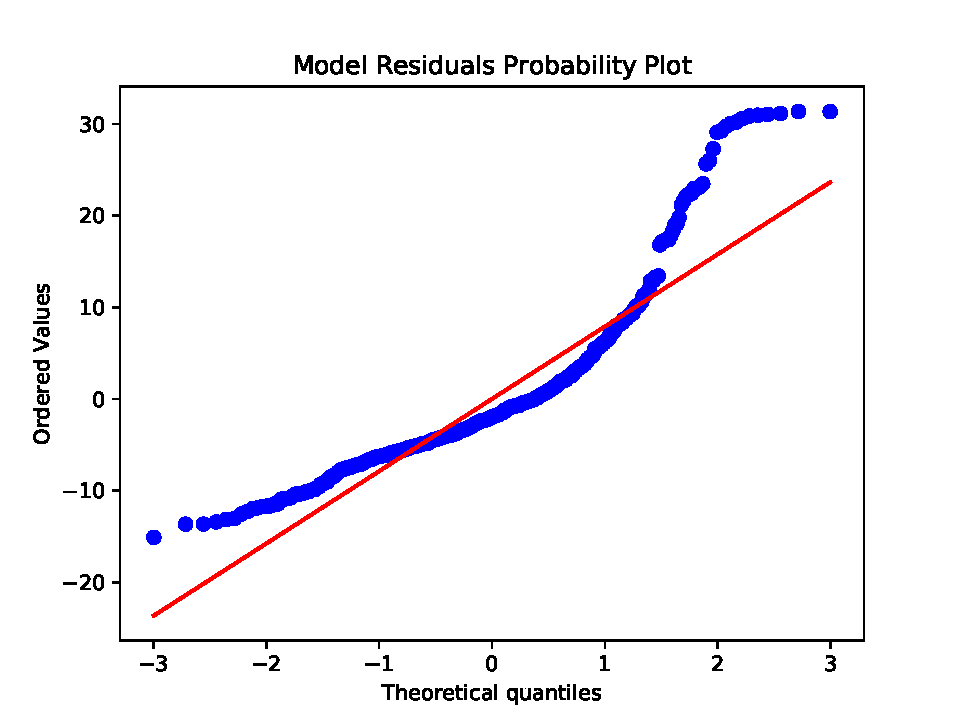
\includegraphics{hw5_1_e.pdf}    

  \item

     Yes and no. We have a significantly significant predictor for age and price, however, we have a low r-squared which suggests that we are not explaining the variance in the model very well. Also, the probability plot and kstest suggests that the model does not have normally distributed residuals. The non-normally distributed residuals suggests some potential pattern in the data the linear model cannot capture.

     I think that the low r-squared could be OK in this scenario, meaning that the housing price has a lot of variance or complexity, and a linear model can't capture this. I would use this predictor over nothing, but would seek out a better predictor, most likely try something non-linear.
     
  \end{enumerate}
  \lstinputlisting[language=Python]{hw5_1.py}

  Output of Regression:
  
  ==============================================================================
  
  Dep. Variable:                      y   R-squared:                       0.142
  
  Model:                            OLS   Adj. R-squared:                  0.140
  
  Method:                 Least Squares   F-statistic:                     83.48
  
  Date:                Thu, 04 Apr 2019   Prob (F-statistic):           1.57e-18
  
  Time:                        17:50:32   Log-Likelihood:                -1801.5
  
  No. Observations:                 506   AIC:                             3607.
  
  Df Residuals:                     504   BIC:                             3615.
  
  Df Model:                           1
  
  Covariance Type:            nonrobust
  
  ==============================================================================
  
  coef    std err          t      P>|t|      [0.025      0.975]
  
  ------------------------------------------------------------------------------
  
  const         30.9787      0.999     31.006      0.000      29.016      32.942
  
  x1            -0.1232      0.013     -9.137      0.000      -0.150      -0.097
  
  ==============================================================================
  
  Omnibus:                      170.034   Durbin-Watson:                   0.613
  
  Prob(Omnibus):                  0.000   Jarque-Bera (JB):              456.983
  
  Skew:                           1.671   Prob(JB):                    5.85e-100
  
  Kurtosis:                       6.240   Cond. No.                         195.
  
  ==============================================================================
  

  
\item
  \begin{enumerate}
  \item
    The covariance matrix for our predictors is
    \[  \begin{bmatrix}
    
        - &     NOX    &        RM   &            DIS &         LSTAT \\
    
    NOX   & 1.      &   -0.30218819  &   -0.76923011 &    0.59087892 \\
    
    RM    & -0.30218819    &   1.    &      0.20524621  &  -0.61380827 \\
    
    DIS   & -0.76923011 &  0.20524621   &        1.   &     -0.49699583 \\
    
    LSTAT & 0.59087892 &  -0.61380827   &  -0.49699583 &    1.
  \end{bmatrix} \]
    

    
\item

  The VIF calculation for each predictor is

  \[ \begin{bmatrix}

      CONSTANT & NOX    &        RM   &            DIS &         LSTAT \\
      
      276.741  & 2.853 & 1.639 & 2.496 & 2.299

    \end{bmatrix} \]

  Multi-collinearity is a problem because coefficient estimates of multiple regression can change erraticaly in response to small changes in the model or data. In perfect multicolinearity, the OLS estimator optimal solutions do not exist. $X^TX$ does not have an inverse. In multicolinearity, X is not full rank.
\item

  Since the VIF values calculated were all under 10, we do not need to drop any predictors for this model. The solution to the linear regression is below.

  OLS Regression Results
  
  ==============================================================================

  Dep. Variable:                      y   R-squared:                       0.659 
  
  Model:                            OLS   Adj. R-squared:                  0.656  
  
  Method:                 Least Squares  \textbf{ F-statistic:                     241.6 }
  
  Date:                Thu, 04 Apr 2019   \textbf{Prob (F-statistic):          2.09e-115 }
  
  Time:                        18:14:47   Log-Likelihood:                -1568.4 
  
  No. Observations:                 506   AIC:                             3147. 
  
  Df Residuals:                     501   BIC:                             3168. 
  
  Df Model:                           4 
  
  Covariance Type:            nonrobust 

  ==============================================================================
  
  coef    std err          t      P>|t|      [0.025      0.975]
  
  ------------------------------------------------------------------------------
  
  const         12.0360      3.990      3.016      0.003       4.196      19.876
  
  x1           -14.5379      3.500     -4.154      0.000     -21.414      -7.662
  
  x2             4.8634      0.438     11.115      0.000       4.004       5.723
  
  x3            -0.9670      0.180     -5.367      0.000      -1.321      -0.613
  
  x4            -0.6587      0.051    -12.917      0.000      -0.759      -0.558
  
  ==============================================================================
  
  Omnibus:                      128.609   Durbin-Watson:                   0.866
  
  Prob(Omnibus):                  0.000   Jarque-Bera (JB):              362.399
  
  Skew:                           1.222   Prob(JB):                     2.02e-79
  
  Kurtosis:                       6.349   Cond. No.                         311.
  
==============================================================================


\item
  The F-statistic was computed and shown in the model summary above. Due to the F-statistic being high, with a very small p-value,  we can reject the null hypothesis. The null hypothesis is that the intercept only model (no predictor variables) is equal to the model with the predictor variables. In other words, our model with the predictor variables gives a better fit than a model with just a y-intercept or at least one predictor coeficient, $\beta_j \neq 0$.


  
  \end{enumerate}

    \lstinputlisting[language=Python]{hw5_2.py}
  
  \item

    \begin{enumerate}
      
    \item
      The OLS results for the model is shown below.
      
      OLS Regression Results
      
      ==============================================================================
      
      Dep. Variable:                      y   R-squared:                       0.229
      
      Model:                            OLS   Adj. R-squared:                  0.226
      
      Method:                 Least Squares   F-statistic:                     74.65
      
      Date:                Thu, 04 Apr 2019   Prob (F-statistic):           4.08e-29
      
      Time:                        18:42:34   Log-Likelihood:                -1774.5
      
      No. Observations:                 506   AIC:                             3555.
      
      Df Residuals:                     503   BIC:                             3568.
      
      Df Model:                           2
      
      Covariance Type:            nonrobust
      
      ==============================================================================
      
      coef    std err          t      P>|t|      [0.025      0.975]
      
      ------------------------------------------------------------------------------
      
      const         41.6722      1.762     23.652      0.000      38.211      45.134
      
      x1             7.8224      1.424      5.494      0.000       5.025      10.620
      
      x2           -35.4798      3.121    -11.369      0.000     -41.611     -29.349
      
      ==============================================================================
      
      Omnibus:                      156.666   Durbin-Watson:                   0.744
      
      Prob(Omnibus):                  0.000   Jarque-Bera (JB):              383.211
      
      Skew:                           1.581   Prob(JB):                     6.12e-84
      
      Kurtosis:                       5.859   Cond. No.                         11.4
      
      ==============================================================================
      


    \item
       $\beta_0$ explains average price of houses not bordering the Charles River.

     \item
       $\beta_1$ explains the average difference between houses that border the Charles river and those that don't.

     \item
       We don't include two dummy variables because then there is a problem with multi-colinearity. If one variable is 0, the other is 1. There is a perfect relationship between them.
Consider that the constant term is a vector of ones. Then, by construction, the two dummy variables will add to be a vector of 1s. This occurs because When a variable is 0, the other is 1 and vice versa. $0 + 1 = 1 + 0 = 1$ Therefore, the intercept is a linear combination of the dummy variables, creating the co-linearity.
    \end{enumerate}

    \lstinputlisting[language=Python]{hw5_3.py}
    
\item
  \begin{enumerate}

  \item
    The value of k used was 5. The plot shows the k-fold cross validation error. 

      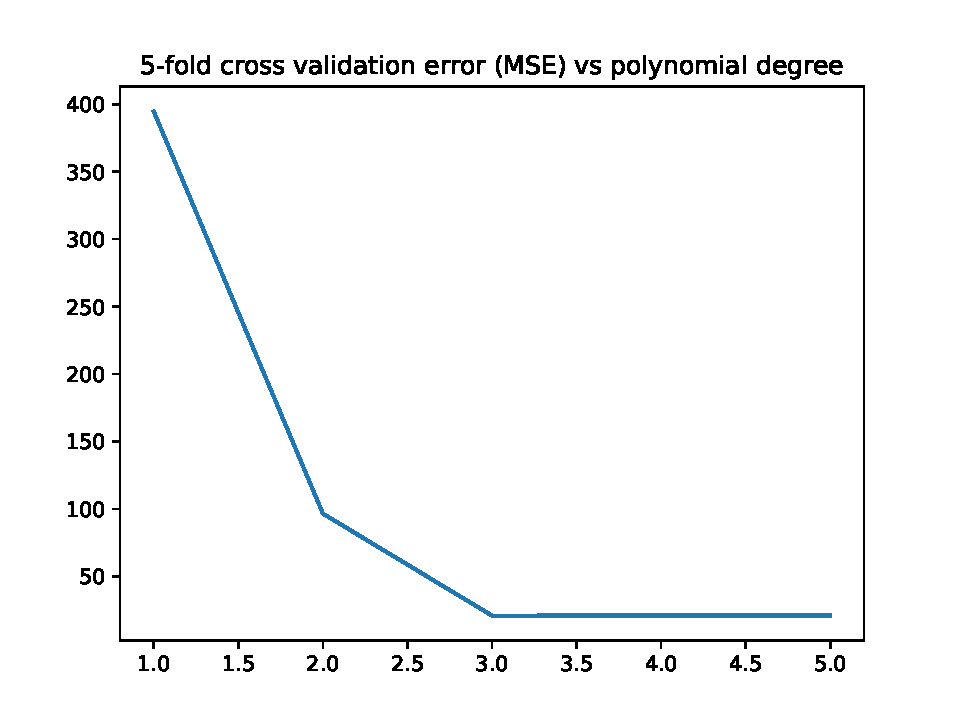
\includegraphics[width=\textwidth]{hw5_4_a.pdf}    
    \item
      I chose the smallest polynomial model (smallest in degree) that gave the lowest MSE. It actually flattened up to around 10, with minor variations or actually increasing. The polynomial with the smallest MSE was a polynomial with degree 3, $\beta_0 + \beta_1x + \beta_2x^2 + \beta_3x^3$. The model results and the fitted polynomial against the labels (with confidence intervals) are plotted below.

      OLS Regression Results
      
      ==============================================================================
      
      Dep. Variable:                      y   R-squared:                       0.947
      
      Model:                            OLS   Adj. R-squared:                  0.946
      
      Method:                 Least Squares   F-statistic:                     1161.
      
      Date:                Thu, 04 Apr 2019   Prob (F-statistic):          1.79e-124
      
      Time:                        20:20:55   Log-Likelihood:                -584.23
      
      No. Observations:                 200   AIC:                             1176.
      
      Df Residuals:                     196   BIC:                             1190.
      
      Df Model:                           3
      
      Covariance Type:            nonrobust
      
      ==============================================================================
      
      coef    std err          t      P>|t|      [0.025      0.975]
      
      
      ------------------------------------------------------------------------------
      
      const         19.7951      0.536     36.941      0.000      18.738      20.852
      

      x1           -19.0345      0.379    -50.192      0.000     -19.782     -18.287
      
      x2            -0.1079      0.279     -0.386      0.700      -0.659       0.443
      
      x3             2.2490      0.084     26.672      0.000       2.083       2.415
      
      ==============================================================================
      
      Omnibus:                        0.116   Durbin-Watson:                   1.954
      
      Prob(Omnibus):                  0.944   Jarque-Bera (JB):                0.206
      
      Skew:                           0.053   Prob(JB):                        0.902
      
      Kurtosis:                       2.883   Cond. No.                         37.5
      
      ==============================================================================
      
      
      
      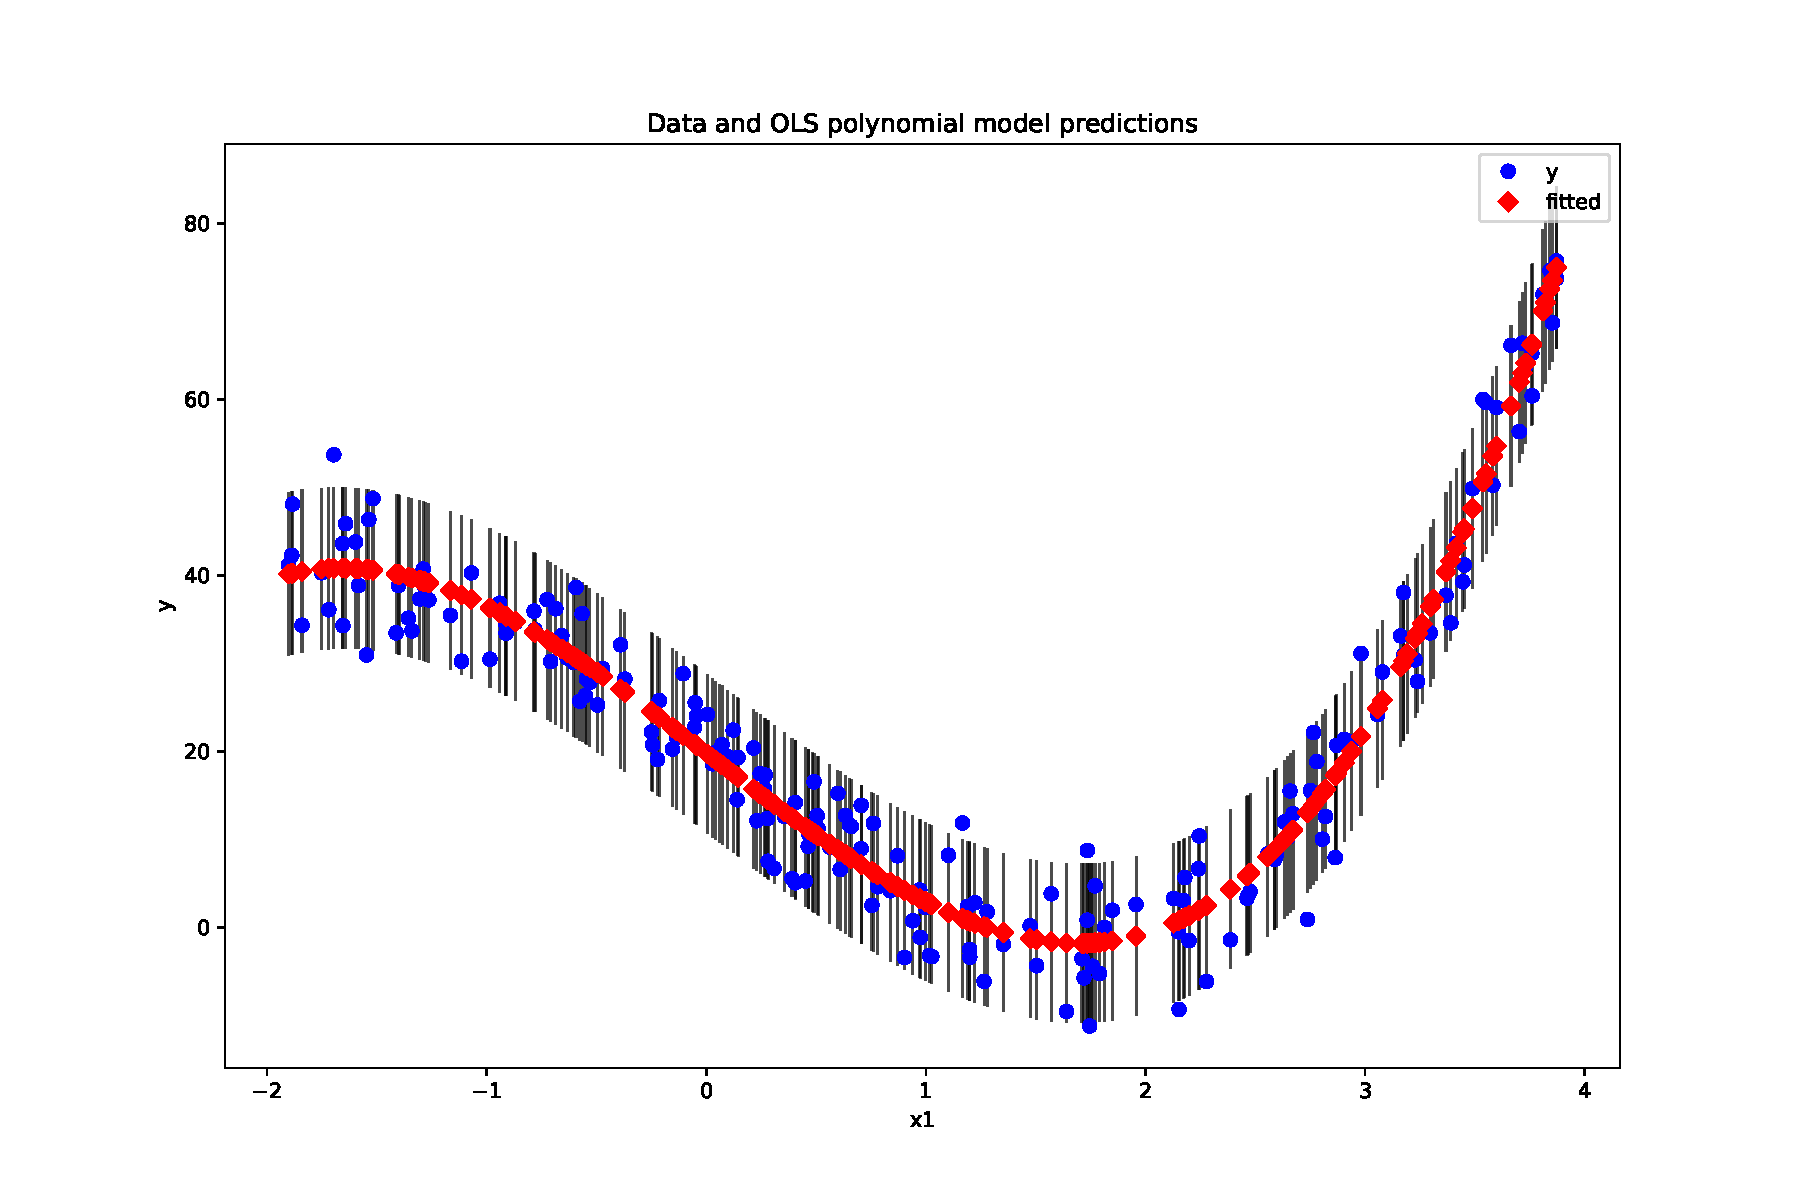
\includegraphics[width=\textwidth]{hw5_4_b.pdf}    

  \end{enumerate}

  \lstinputlisting[language=Python]{hw5_5.py}
  
\end{enumerate}

\end{document}

%=========================== END DOCUMENT ==============================

